\chapter{Introdução}
Este manual tem como objetivo mostrar o uso das ferramentas
do InVesalius e também apresentar alguns conceitos para facilitar
a utilização do software.

O InVesalius é um software para auxiliar o profissional
de saúde no diagnóstico	e no planejamento cirúrgico. Cabe
ressaltar, porém, que todo software no contexto de diagnóstico é
totalmente suplementar, pois todo e qualquer ato cometido é de
inteira responsabilidade do profissional de saúde.

Além da medicina, é possível utilizar o software em outras áreas, como
arqueologia, veterinária, ou mesmo em aplicações industriais.
Como requisito básico, basta que as imagens a serem analisadas
estejam no padrão DICOM (\textsl{Digital Imaging Communications in Medicine}).
Até o presente momento, o InVesalius reconstrói
imagens provindas de tomógrafos e de aparelhos de ressonância magnética.
Para operar o software, basta ter conhecimentos básicos de 
informática. Noções básicas sobre imagens médicas podem contribuir para o
melhor entendimento das operações.


\section{Conceitos importantes}
Nesta seção, discutiremos alguns conceitos necessários para melhor
entendimento e operação do software.


\subsection{DICOM (\textit{Digital Image Communications in Medicine})}			
DICOM é um padrão relativo à transmissão, ao armazenamento e
ao tratamento de imagens médicas. O padrão prevê diversas modalidades de imagens médicas,
como imagens provindas de equipamentos de tomografia computadorizada, ressonância magnética,
ultrassom, eletrocardiograma, entre outras.

Uma imagem DICOM é composta por 2 itens principais, uma matriz contendo os pixels da
imagem e um conjunto de meta-informações. Essas informações contêm, por exemplo, o nome
do paciente, a modalidade da imagem e a posição da imagem em relação ao espaço (no caso
de tomografia e ressonância).


\subsection{Tomografia Computadorizada - Médica}
A tomografia computadorizada indica a radiodensidade dos tecidos, isto é, a média de
absorção de raios-X pelos tecidos. A radiodensiade é traduzida para a imagem em níveis
de cinza em uma escala chamada \textit{Hounsfield}, nome dado em homenagem a Godfrey
Newbold Hounsfield, um dos criadores da primeira máquina de tomografia computadorizada.

%\begin{wrapfigure}{c}{0.5\textwidth}
%  \begin{center}
%    \includegraphics[scale=0.3]{img/tomografo.jpg}
%  \end{center}
%  \caption{Tomógrafo Médico http://www.toshibamedical.com.br}
%\end{wrapfigure}
\begin{figure}[!htb]
\centering
\includegraphics[scale=0.4]{tomografo.jpg}
\caption{Tomógrafo médico - www.toshibamedical.com.br}
\end{figure}

%\begin{figure}[!htb]
%\centering
%\includegraphics[scale=0.3]{img/tomografo.jpg}
%\caption{Tomógrafo Médico}
%\end{figure}

Nos aparelhos mais modernos, com um emissor de radiação e um banco de
sensores (também chamados de canais, variando de 2 até 256), que circundam o paciente
enquanto a maca é movimentada, formando uma espiral, é possível gerar uma
grande quantidade de imagens, simultaneamente, com pouca emissão de raios-X.


\subsubsection{Escala de Hounsfield}
Como citado na seção anterior, as imagens de tomografia computadorizada
são geradas em níveis de cinza, os quais são depois traduzidos na escala
de Hounsfield (HU). Os tons mais claros representam tecidos mais densos, e
os mais escuros, tecidos menos densos, como a pele e o cérebro.
A tabela \ref{tab:escala_hounsfield} apresenta alguns materiais e seus 
respectivos valores em HU (\textit{Hounsfield Unit}).


\begin{table}[h]
\centering
\caption{Escala de Hounsfield}
\begin{tabular}{lcc}\\
\hline % este comando coloca uma linha na tabela
Material & HU\\
\hline
\hline
Ar & -1000 ou menos\\
Gordura & -120\\
Água & 0\\
Músculo & 40\\
Contraste & 130\\
Osso & 400 ou mais\\
\hline
\end{tabular}
\label{tab:escala_hounsfield}
\end{table}


\subsection{Tomografia Computadorizada - Odontológica}

A tomografia computadorizada odontológica comumente trabalha com menos emissão
de radiação se comparada à tomografia computadorizada médica e, em consequência,
torna possível visualizar mais detalhes de regiões delicadas, como a cortical alveolar.

\begin{figure}[!htb]
\centering
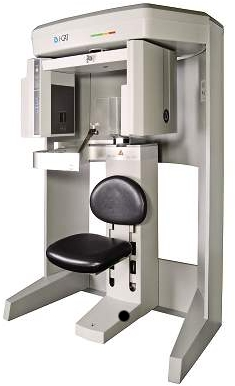
\includegraphics[scale=0.4]{feixe_conico.jpg}
\caption{Tomógrafo odontológico - www.kavo.com.br}
\end{figure}

A aquisição das imagens é feita com o paciente na vertical (ao contrário da tomografia médica,
em que o paciente fica na horizontal). Um emissor e um sensor de raios-X circundam o crânio
do paciente, formando um arco de $180^\circ$ ou $360^\circ$. As imagens geradas pelo tomógrafo
podem ser interpretadas como um volume com o crânio do paciente imerso. Esse volume é "fatiado"
pelo software do aparelho, podendo-se gerar imagens com espaçamentos diferentes ou outros
tipos de imagens, como a visão panorâmica da região de interesse.

As imagens adquiridas por tomógrafos odontológicos costumam exigir um maior pós-processamento
quando é necessário separar (segmentar) determinadas estruturas usando outros softwares como
o InVesalius. Isso ocorre porque, normalmente, essas imagens possuem mais níveis de cinza que
a escala de Hounsfield, o que torna o uso de padrões de segmentação \textit{(presets)} menos
eficiente. Outra característica bastante comum nas imagens provindas de tomógrafos
odontológicos é a alta presença de ruídos do tipo \textit{speckle} e a presença de outros
ruídos normalmente causados por uso de próteses de amálgama pelo paciente.


\subsection{Ressonância Magnética}

A ressonância magnética é um exame realizado sem o uso de radiação ionizante. Em vez disso,
é utilizado um forte campo magnético para alinhar os átomos de algum elemento presente em
nosso corpo, comumente o hidrogênio. Após o alinhamento, são disparadas ondas de rádio, e os
átomos são excitados. Os sensores medem o tempo que os átomos de hidrogênio demoram para se
alinhar novamente. Com isso, é possível determinar qual é o tipo de tecido, pois tecidos
diferentes apresentam quantidades diferentes de átomos de hidrogênio.

Para evitar interferências e melhorar a qualidade do sinal de radiofrequência, além de o
paciente ficar dentro do equipamento, é colocada uma bobina na região de interesse.

 
\begin{figure}[!htb]
\centering
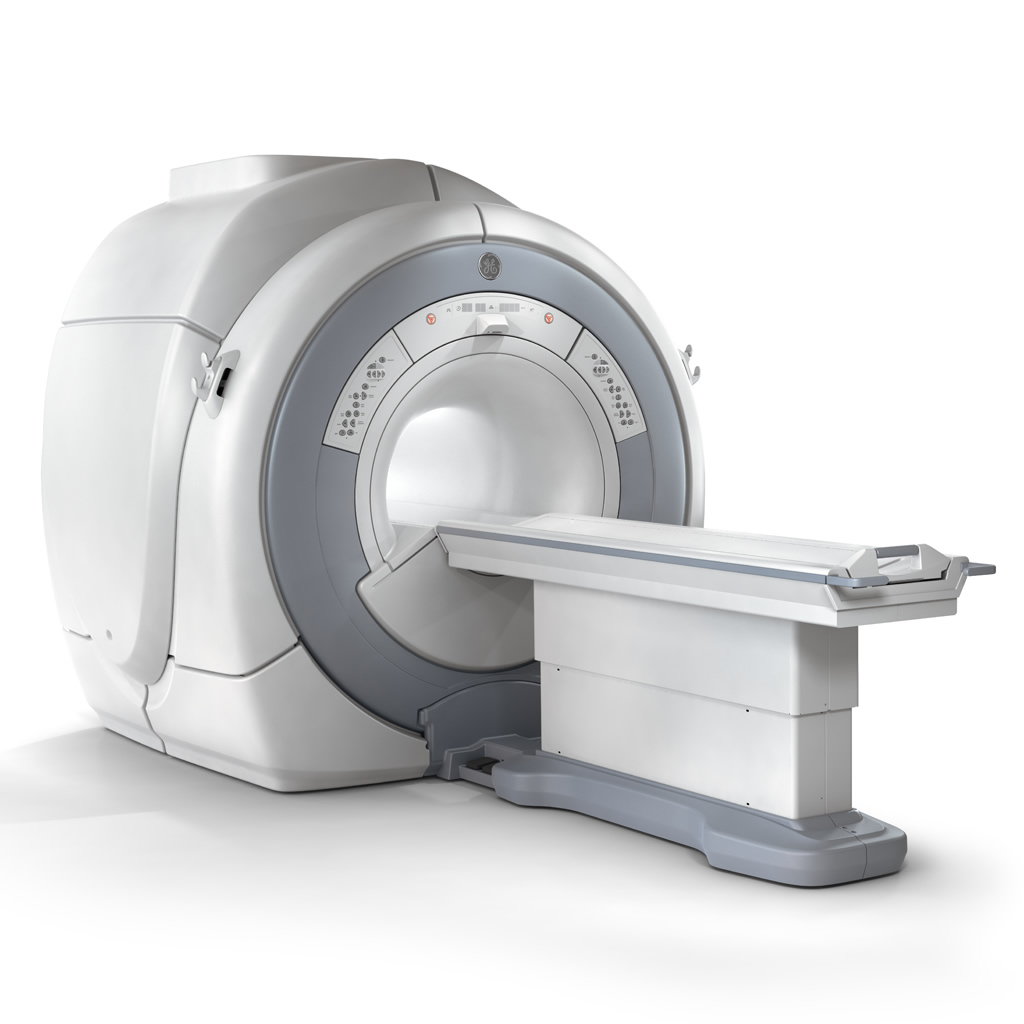
\includegraphics[scale=0.2]{rm_ge.jpg}
\caption{Equipamento de ressonância magnética - www.gehealthcare.com}
\end{figure}

\begin{figure}[!htb]
\centering
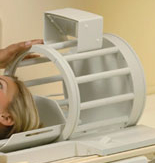
\includegraphics[scale=0.8]{bobina.jpg}
\caption{Bobina - www.healthcare.philips.com}
\end{figure}

\subsection{Neuronavegação}
\label{sec:neuronavegador_intro}

Neuronavegação é a uma técnica que permite localizar e rastrear instrumentos cirúrgicos em relação às estruturas neuronais através da visualização computacional. Além disso, sistemas de neuronavegação têm sido apontados como uma ferramenta fundamental para estudos em planejamento pré-cirúrgico e aumentar a precisão de experimentos em neurociência, como a estimulação magnética transcraniana (EMT), eletroencefalografia (EEG), magnetoencefalografia (MEG) e espectroscopia no infravermelho próximo. Apesar do vasto campo de aplicações, o uso da neuronavegação em centros de pesquisa é limitado pelo alto custo. O módulo de neuronavegação do InVesalius oferece aos usuários uma alternativa de baixo custo e código aberto aos sistemas comercias de navegação. Desta maneira, é possível utilizar ferramentas específicas para neuronavegação e ainda ter a possibilidade de desenvolvimento de funcionalidades sob demanda. O neuronavegador é distribuído em uma versão executável compatível com sistemas operacionais Windows 7, 8 e 10.. O capítulo~\ref{sec:neuronavegador}, apresenta detalhes sobre o uso desta ferramenta.


\section{Recursos necessários}
O InVesalius é projetado para executar em computadores pessoais, como
\textit{desktops} e \textit{notebooks}. Atualmente, ele é compatível com
os seguintes sistemas operacionais:\\
- MS-Windows (Windows 7, 8 e 10)\\
- GNU/Linux (Ubuntu, Mandriva, Fedora)\\
- Apple Mac OS X

O desempenho do InVesalius depende, principalmente, da quantidade de fatias
reconstruídas (imagens abertas pelo software), da quantidade de memória RAM
disponível, da frequência do processador e da arquitetura do sistema operacional
(32 \textit{bits} ou 64 \textit{bits}).

Vale ressaltar, como regra geral, que quanto maior a quantidade de memória RAM
disponível no sistema, maior será o número de fatias que podem ser abertas
simultaneamente para um dado estudo. Por exemplo, com 1 GB de memória disponível,
pode-se abrir cerca de 300 fatias com resolução de 512x512 \textit{pixels}.
Já com 4 GB de memória, pode-se abrir em torno de 1000 imagens com a mesma
resolução.

			
\subsection{Configurações mínimas}
Sistema Operacional de 32 \textit{bits}\\
Processador Intel Pentium 4 ou equivalente, com frequência de 1,5 GHz\\
1 GB de memória RAM\\
80 GB de disco rígido\\
Placa gráfica com 64 MB de memória\\
Resolução de vídeo de 1024x768 \textit{pixels}


\subsection{Configurações recomendadas}
Sistema Operacional de 64 \textit{bits}\\
Processador Intel Core 2 Duo ou equivalente, com frequência de 2,5 GHz\\
4 GB de memória RAM\\
180 GB de disco rígido\\
Placa gráfica NVidia ou ATI, com 128 MB de memória\\
Resolução de vídeo de 1024x768 \textit{pixels}

